\documentclass{article}
\usepackage{amsmath}
\usepackage{tikz}
% \usepackage{esvect}
\usepackage{cancel}
\usepackage{float}
\usepackage{comment}

\newcommand{\dd}[2]{\frac{\mathrm{d}#1}{\mathrm{d}#2}}
\newcommand{\vv}[1]{\overline{#1}}

\pagestyle{empty}
\begin{document}

% \section*{Diagrams}
The circular restricted three body problem (CR3BP) is a special case of the three body problem. In the CR3BP (much like in Keplerian 2-body dynamics), we neglect the mass of satellite $S$, while treating the larger celestial body $B_1$ and smaller celestial body $B_2$ as point masses. Crucially, these bodies must orbit one another in circular orbits. In other words, they both orbit about their inertially fixed barycenter $c$ \textit{at constant velocity and distance}.
\begin{figure}[H]
    \centering
    \begin{tikzpicture}[
        planet/.style = {circle, draw=black, ball color=#1, node contents={}, inner sep = 0.1cm}, 
        point/.style = {circle, draw=#1, fill=#1, node contents={}, inner sep=0.05cm},
        >=latex
        ]

        \draw[dotted, fill=none, green](0,0) circle (1);
        \draw[dotted, fill=none, blue](0,0) circle (3);
        \node (B1) at (-1,0)     [planet=green, label=left:$B_1$];
        \node (B2) at (3,0)      [planet=blue, label=right:$B_2$];

        \draw[dashed, green] (B1) -- (0,0) node[midway, below] {$x_1$};
        \draw[dashed, blue] (0,0) -- (B2) node[midway, below] {$x_2$};
        
        \node (o) at (0,0)      [point=black, label=below:$c$];
        \node (r) at (1.5,0.75)    [point=red, label=left:$S$];
        \draw[->, gray] (0,0) -- (0.75,0) node[near end, above] {$\hat{x}$};
        \draw[->, gray] (0,0) -- (0,0.75) node[near end, left] {$\hat{y}$};
    \end{tikzpicture}

    \caption{Geometry. $S$ is the satellite, $B$ are the celestial bodies. $\hat{z}$ implied out of page. The bodies are always along the $x$ axis, as the $c$ frame rotates with them}
\end{figure}

\begin{comment}
\begin{figure}[H]
    \centering
    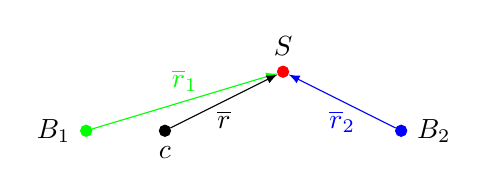
\begin{tikzpicture}[
        point/.style = {circle, draw=#1, fill=#1, node contents={}, inner sep=0.05cm},
        >=latex
        ]

        \node (B1) at (-1,0)     [point=green, label=left:$B_1$];
        \node (B2) at (3,0)      [point=blue, label=right:$B_2$];
        \node (o) at (0,0)      [point=black, label=below:$c$];
        \node (S) at (1.5,0.75)    [point=red, label=above:$S$];

        \draw[->, blue] (B2) -> node[below] {$\vv{r}_2$} (S);
        \draw[->, green] (B1) -> node[above] {$\vv{r}_1$} (S);
        \draw[->, black] (o) -> node[below] {$\vv{r}$} (S);
    \end{tikzpicture}
    \caption{Vectors. Note $x_1$ refers to the distance from $c$ to $B_1$ and $x_2$ refers to the distance from $c$ to $B_2$. Predictably, $r_{12}=x_1+x_2$ is the distance between the bodies}
\end{figure}
\end{comment}

Because $\hat{x}$ points from $c$ to $B_2$, which is not inertially stationary, the $xyz$ frame is rotating. Specifically, it is rotating positively about $z$. Because the celestial bodies are in a circular orbit, their rates of rotation about $c$ are constant. This means that the $xyz$ frame rotates at a constant rate of $\vv{\omega}=\Omega\hat{z}$ 

We can also find a relationship between $x_1$, $x_2$, $r_{12}$, $m_1$, and $m_2$. Because $c$ is the barycenter,
\[\boxed{x_1m_1=x_2m_2}\]

\section*{Kinematics}
The transport theorem states that the inertial (fixed $f$ frame) derivative of a vector $u$ (expressed in the rotating $c$ frame) is

\[\dd{^f \vv{u}}{t}=\dd{^c\vv{u}}{t}+\vv{\omega}^{cf}\times\vv{u}\]

Where $\dd{^f}{t}$ denotes the derivative in the coordinates of the fixed frame $f$, and $\dd{^c}{t}$ denotes derivative in the coordinates of the rotating frame $c$, and $\vv{\omega}^{cf}$ denotes the angular velocity of $c$ in $f$. For this case, $\vv{\omega}^{cf}=\Omega\hat{z}$.


For a position vector $\vv{r}$, we will find the velocity $\vv{v}=\dot{\vv{r}}$ and acceleration $\vv{a}=\ddot{\vv{r}}$. Note that dot notation implies inertial. 

\[
\begin{aligned}
    \vv{v}&=\dot{\vv{r}}\\
    &=\dd{^c\vv{r}}{t}+\vv{\omega}^{cf}\times\vv{r}\\
    &=\vv{v}^c+\left(\Omega\hat{z}\times\vv{r}\right)
\end{aligned}
\]

\[
\begin{aligned}
    \vv{a}&=\dot{\vv{v}}\\
    &=\dd{^c}{t}\left(\vv{v}^c+\left(\Omega\hat{z}\times\vv{r}\right)\right)+\vv{\omega}^{cf}\times\left(\vv{v}^c+\left(\Omega\hat{z}\times\vv{r}\right)\right)\\
    &=\dd{^c}{t}\left(\vv{v}^c+\left(\Omega\hat{z}\times\vv{r}\right)\right)+\Omega\hat{z}\times\left(\vv{v}^c+\left(\Omega\hat{z}\times\vv{r}\right)\right)\\
    &=\vv{a}^c+\left(\Omega\hat{z}\times\vv{v}^c\right)+\Omega\hat{z}\times\left(\vv{v}^c+\left(\Omega\hat{z}\times\vv{r}\right)\right)\\
    &=\vv{a}^c+\left(\Omega\hat{z}\times\vv{v}^c\right)+\left(\Omega\hat{z}\times\vv{v}^c\right)+\Omega\hat{z}\times\left(\Omega\hat{z}\times\vv{r}\right)\\
    &=\vv{a}^c+2\left(\Omega\hat{z}\times\vv{v}^c\right)-\Omega^2\vv{r}\\
\end{aligned}
\]

\[\boxed{\vv{v}=\vv{v}^c+\left(\Omega\hat{z}\times\vv{r}\right)}\]
\[\boxed{\vv{a}=\vv{a}^c+2\left(\Omega\hat{z}\times\vv{v}^c\right)}\]

Now we will solve for $\Omega$. Note that, because $c$ is the center of mass of $B_1$ and $B_2$, 

\[\begin{aligned}
    F_{\text{on2}}&=-\frac{Gm_1m_2}{r_{12}^2}\hat{x}\\
    \cancel{m_2}\vv{a}_2^f&=-\frac{Gm_1\cancel{m_2}}{r_{12}^2}\hat{x}\\
    \left(\cancelto{0}{\vv{a}^c}+2\left(\Omega\hat{z}\times\cancelto{0}{\vv{v}^c}\right)-\Omega^2\vv{r}\right)&=\frac{Gm_1}{r_{12}^2}\\
    -\Omega^2x_2\hat{x}&=-\frac{Gm_1}{r_{12}^2}\hat{x}\\
    \Omega^2x_2&=\frac{Gm_1}{r_{12}^2}\\
    \Omega&=\sqrt{\frac{Gm_1}{x_2r_{12}^2}}\\
\end{aligned}\]

\end{document}
